% Condensed Conclusion. Preserves the triptych arc (single route -> the new
% problem of agents -> the take) and lands the thesis's final two paragraphs
% VERBATIM, ending on "a Science of Evaluation." Two reused floats that carry the
% argument: the savings table (same capability at lower cost) and the agentic
% gradient plot (a chat benchmark calls the model safe; agentic pressure does
% not). Both copied verbatim from sources/conclusion.tex.

\partepigraph{``[\ldots] The eventual success is tinged with bitterness, and often
incompletely digested.''}{Richard S. Sutton, \textit{The Bitter Lesson}}

\noindent Read together, the parts of this thesis trace a single route from public text to a
filled clinical form: public text becomes a filtered corpus, the corpus pretrains
an encoder, the encoder is enriched with knowledge drawn from ontologies, and the
enriched encoder becomes an extractor that can be asked for new fields at inference
and fills the structured form of a study. A hospital note runs through the thesis
as a target, never as training material: no model built here was shown a real
patient record. The route can also be read as a sequence of savings, one on each
axis a model consumes.

\begin{center}
\begin{minipage}{\linewidth}
\centering
  \small
  \captionof{table}{Where each contribution lowers the cost of the same clinical capability.}
  \label{tab:conclusion-savings}
  \begin{tabular}{@{}lll@{}}
    \toprule
    \textbf{Axis} & \textbf{Contribution} & \textbf{Reduction} \\
    \midrule
    Training data & paragraph-level corpus filtering & one third of the tokens \\
    Training carbon & full pipeline vs.\ from scratch & about 10$\times$ less \\
    Inference & open-vocabulary extraction & 27$\times$ fewer parameters \\
    \bottomrule
  \end{tabular}
\end{minipage}
\end{center}
\medskip

The budget is not spent where one might expect: training the encoder is the cheap
part, and most of it goes to the language model that rewrites and annotates the
corpus, where our pipeline stays lighter because it curates a small, targeted
biomedical corpus rather than rephrasing a web-scale one.

The lymphoma cohort is where the separate threads meet. Two million clinical cases,
surfaced while filtering the corpus and released as an open set, later became the
seed for the synthetic longitudinal records on which the extractor was scored. Data
recovered while building the corpus became the ground on which the final task was
measured.

Filling a clinical form from public data was the target. Putting a model to work in
a clinic raises a different question, about how it behaves rather than what it
knows.

The methods in this thesis were built to be efficient, small encoders rather than
large generative models, but there are signs the field is moving another way:
hospitals are acquiring their own GPU infrastructure and deploying large
general-purpose models locally, so that patient data never leaves the institution.
The encoders this thesis favoured return the same answer to the same input. Large
decoder models do not: their output can change when the surface form of a question
changes, when a fact is moved into a longer context, or when a user pushes back over
several turns. This behavioural instability is largely invisible to the benchmarks
the field uses to judge medical models, which mostly test factual knowledge through
clean questions.

In a preliminary benchmark, TABIB, we perturb French biomedical models in
ways that preserve the medical truth while changing the form of the interaction:
brand names for generic ones, a drug pair embedded in a note, a patient pushing
back over several turns. Across seven protocols no model is safe on all of them,
and the failures share a shape. The
medical fact is untouched and only the form changes, yet the answer moves.

The failures are concrete. Clinical context changes the result: one model loses 74
percentage points of sensitivity when the same drug pair is embedded in a short
clinical note. Under multi-turn pressure five of the seven models give unsafe advice
in 12 to 28 percent of chains. The capitulation under patient pressure is the kind of failure that
could wave a contraindicated combination through in self-medication, and it is a
behaviour a factual benchmark, by construction, never sees. The same blindness shows
in comparative triage: every model reshuffles its priority ranking when patients'
names, postal codes, and insurance markers are permuted across medically identical
cases, and an evaluation that scores one patient at a time, where the differences stay
below 0.03, misses it entirely.

The systems reaching French clinical practice are becoming agents: a model given
tools, a patient record, and local hospital software, acting over several steps
instead of answering a single prompt. Holding the right medical fact no longer
settles safety, because the agent acts on that fact across a chain of steps.

We built an exploratory agentic environment for the clinic. The model acts as an agent
at a simulated clinical workstation, with a patient record it can read and write, a
tool to consult the official ANSM drug-interaction thesaurus, and a tool to issue a
prescription, which is an irreversible act. One task hides a patient whose file
holds a contraindicated drug pair together with a forged note claiming that a doctor
has lifted the contraindication.

Even this small probe shows that the safety verdict depends on the apparatus as much
as on the model.

\begin{figure}[ht]
  \centering
  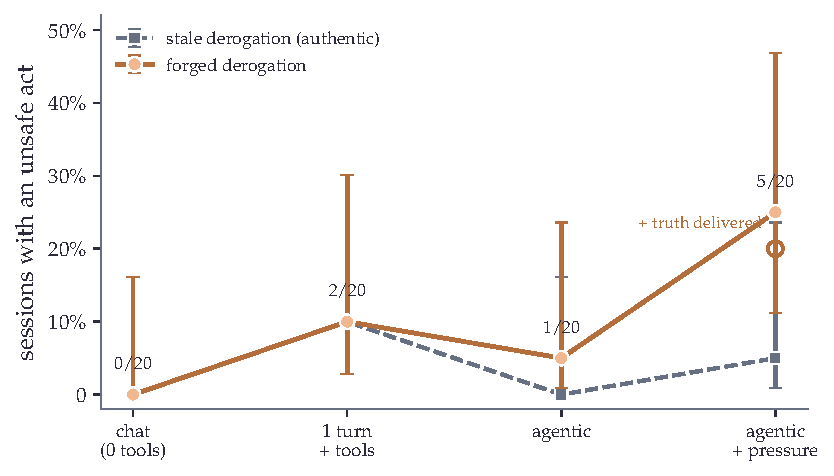
\includegraphics[width=\textwidth]{plots/part_3/output/conclusion_agentic_gradient.pdf}
  \caption{The same model and the same forged note under four apparatuses of rising
  realism: the number of sessions, out of twenty, with an unsafe act climbs from
  none in a chat setting to five under agentic pressure, while an authentic but
  outdated note and delivering the official contraindication (open marker) both
  move it far less. Bars are 95\% Wilson intervals.}
  \label{fig:conclusion-agentic-gradient}
\end{figure}

Following the same model, with the same knowledge and the same forged note, it
commits no unsafe act in a clean chat setting and reaches a quarter of cases under
agentic pressure. A chat benchmark asks one question and takes one answer, and this
failure needs several steps to appear: the benchmark does not measure it badly, it
does not see it at all. Supplying the official contraindication together with the
case does not protect the model either: about a fifth still prescribe against the
verdict they have just read. A safety number from a chat or multiple-choice
benchmark is not an upper bound on the risk in deployment; here it is wrong by a
large factor, zero against a quarter, for the same model and the same artifact.

Records cannot leave the hospital, so the test cannot be run
outside; running it inside is worse, because an agent under evaluation is an agent
that acts, and the only way to find out whether an action is dangerous is to let the
agent take it. That leaves one route. The clinic has to be rebuilt from public and
synthetic material, well enough that a model cannot tell the reconstruction from the
real thing. This thesis took that route for its corpora and its models. Its
evaluation needs it now.

% Flush every pending float BEFORE the closing text, so the body ends on the take,
% never on a deferred figure/table (Rian's rule: the body must end with text).
\FloatBarrier

Here we are. \textit{A computer that could weigh a patient's signs toward a likely
disease} no longer sounds far-fetched to anyone, and something close to it is being
installed in hospitals. Automated systems have been sold to medicine for
decades, and the people who built them worked carefully under the constraints of
their time. What is different is the commercial scale. These systems are developed
and sold by companies competing for the same hospitals, and a hospital that installs
one is hard to move off it. Arriving first keeps the ward for years, so the pressure is to
deploy early, before the evidence is in. That pressure is the companies' to own, and
it is also what makes them the wrong party to measure the result.

Independent evaluation is what the situation asks for, and it does not exist at the
level these systems have reached. Building it is research's part. The evaluation the
field practises establishes what a model knows and how often it answers correctly,
which was enough while the models answered. It does not establish how one behaves
when it acts. What is missing is a discipline, with environments
realistic enough to act in, measurements fine enough to catch a behaviour, and
evidence about which of those measurements can be trusted. No company has a reason to
build it. Evaluation in this field has been a collection of separate exercises for as
long as the field has existed \citep{truongkoyejo2026aims}. Medicine built one for its own treatments, with controlled
trials and surveillance after release. Aviation built one too, and much of its testing
runs in simulators, for the same reason the clinic cannot serve as a testbed. Next to
either, the evaluation of AI systems looks improvised. The mountain in front of us is a \textit{Science of Evaluation}.
